\chapter{Methodological Background}\label{methods}

This Chapter is divided into a number of sections that explore different facets of NLP relevant to this thesis. The first section provides a very brief overview of NLP in general and discusses subjects mentioned later like neural networks, language models, tokenization, and embeddings. The next section delves into the concept of transformers, which have revolutionized the field of NLP by enabling state-of-the-art performance on various language tasks. The discussion of pre-trained language models follows, which have gained popularity in recent years as a result of their outstanding results on a variety of language tasks. Several pre-trained language models, ELMo \citep{peters2018elmo}, GPT \citep{radford2018gpt}, BERT \citep{devlin2018bert}, ELECTRA \citep{clark2020electra}, and T5 \citep{xue2020mt5}, are introduced. The Chapter then covers various semantic search techniques, SBERT \citep{reimers2019sbert}, BERT-Flow \citep{li2020bertflow}, Whitening \citep{huang2021whiteningbert}, SBERT-WK \citep{wang2020sbertwk}, and IS-BERT \citep{zhang2020isbert}, which are used to extract relevant information from texts. The Chapter ends with a section on input pattern design, which discusses how to format input for NLP models to produce predictions.

\section{Natural Language Processing}

NLP is a branch of Artificial Intelligence (AI) that focuses on instructing computers to understand, interpret, and generate human language. The fundamental ideas and methods of NLP, such as neural networks, tokenization, and embeddings, are briefly introduced in the sections that follow.

\subsection*{Neural Networks}

Adapted from the design and function of the human brain, Neural Networks (NNs) are a specific kind of machine learning model. Neural networks are made up of interconnected layers of nodes that process and transform data. Each node receives input from the previous layer's nodes and applies a non-linear function of the sum of its inputs to produce an output that is passed on to the nodes in the next layer. The weights of the connections between the nodes are adjusted during training to reduce the error between the predicted and true outputs. As a result, the NN can recognize patterns and relationships in the data and use them to accurately predict or categorize new data.

\subsection*{Language Models}

Language models (LMs) are models that focus on comprehending and/or producing human language. To learn the statistical patterns and structures of language, LMs are trained on massive amounts of text data, such as books, articles, and web pages. A wide range of tasks, including text generation, machine translation, sentiment analysis, question-answering, and more, can be performed using LMs. They serve as a foundation for comprehending and processing human language in a way that closely resembles human cognition, making them a crucial component of many NLP applications.

\subsection*{Tokenization}

Tokenization is the process of breaking down text into smaller units, called tokens, which can be individual words, subwords, or even special tokens such as end-of-sentence markers. Tokens are the basic building blocks of text and are used as input to various NLP algorithms. For instance, in the sentence ``I love natural language processing'', tokenization might result in tokens such as ``I'', ``love'', ``natural'', ``language'', and ``processing''. Tokens offer a way to represent text in a structured format that NLP algorithms can easily process and analyze. Tokenization is an essential step in many NLP tasks because it lays the groundwork for additional text analysis and processing.

\subsection*{Embeddings}

Because NLP models need numerical representations to process the data, text data cannot be directly input into these models. Here is where embeddings come into play. Word embeddings, sentence embeddings, and document embeddings are numerical representations of text that capture the context and meaning of the text in a continuous vector space. In order for algorithms to effectively analyze, comprehend, and produce human language, these embeddings act as a link between the unstructured text data and the structured numerical data that NLP models can process. One key property of good embeddings is that similar words should have embeddings that are close to each other in the vector space. For instance, words like ``cat'' and ``dog'' should be closer to one another in an embedding space than ``cat'' and ``language''. For many NLP tasks, the similarity or relatedness between words must be captured, and this proximity in the embedding space does just that.


\section{Transformers}\label{transformers}

Moving forward to discuss an important LM architecture, let us delve into the concept of transformers. LMs, as previously stated, are machine learning models that seek to comprehend text in natural languages. Because natural language contains complex and long-term dependencies that go beyond the single word the model is looking at, they need some sort of memory to store and retrieve data in order to carry out this task. The models are only able to produce contextually appropriate responses by keeping track of previously read text. Memory also enables LMs to deal with ambiguity and uncertainty by taking various interpretations of a given text into account (given what has happened before). Without memory, LMs would struggle to capture the variety and complexity of human language.

RNNs (Recurrent Neural Networks) \citep{elman1990rnn}, LSTMs (Long Short-Term Memory) \citep{hochreiter1997lstm}, or GRUs (Gated Recurring Units) \citep{cho2014gru} are different ways to introduce some sort of artificial memory into a model.

The self-attention mechanism that is used for transformers in ``Attention is all you need'' \citep{vaswani2017attention} is another way to enable memory. Attention as a concept was first introduced by \citet{bahdanau2014neural}. Unlike other mechanisms, attention has (in theory) an infinite window of memory, i.e. it doesn't suffer from long-term memory loss. It enables the model to remember everything that might be important, no matter how long ago it was processed. The goal of attention is to find the relevant parts of the input. In order to, for example, translate a sentence, some words are more important than others for predicting the target word. The model needs to learn what these words are and pay more attention to them.

Following the architecture in \citet{vaswani2017attention} the attention mechanism has three key components: the query $q$, the key $k$ and the value $v$.
An answer on Stackoverflow by the user \citet{stackoverflow_attention} gives a good analogy: ``The key/value/query concept is analogous to retrieval systems. For example, when you search for videos on Youtube, the search engine will map your query (text in the search bar) against a set of keys (video title, description, etc.) associated with candidate videos in their database, then present you the best matched videos (values).''

Since attention is calculated on a set of queries simultaneously, the vectors $q, k$ and $v$ become the matrices $Q, K$ and $V$. The query and key matrices then undergo dot product matrix multiplication to produce a score matrix. This matrix has a score for each word pair that determines how much focus should be put on that word when looking at the other word. After scaling the matrix $Q K^T$ and using a softmax, it consists only of values between 0 and 1 that determine the amount of attention for every word. This attention matrix is then multiplied with the values $V$ to get the output. The following matrix notation shows the full formula to get the embeddings using attention from $Q, K$ and $V$ ($d_K$ is the dimension of $K$ used for scaling):

\begin{equation}
\text{Attention(Q,K,V)} = \text{softmax}\left(\frac{Q K^T}{\sqrt{d_K}} \right)V
\end{equation}

\begin{figure}[h!]
\centering
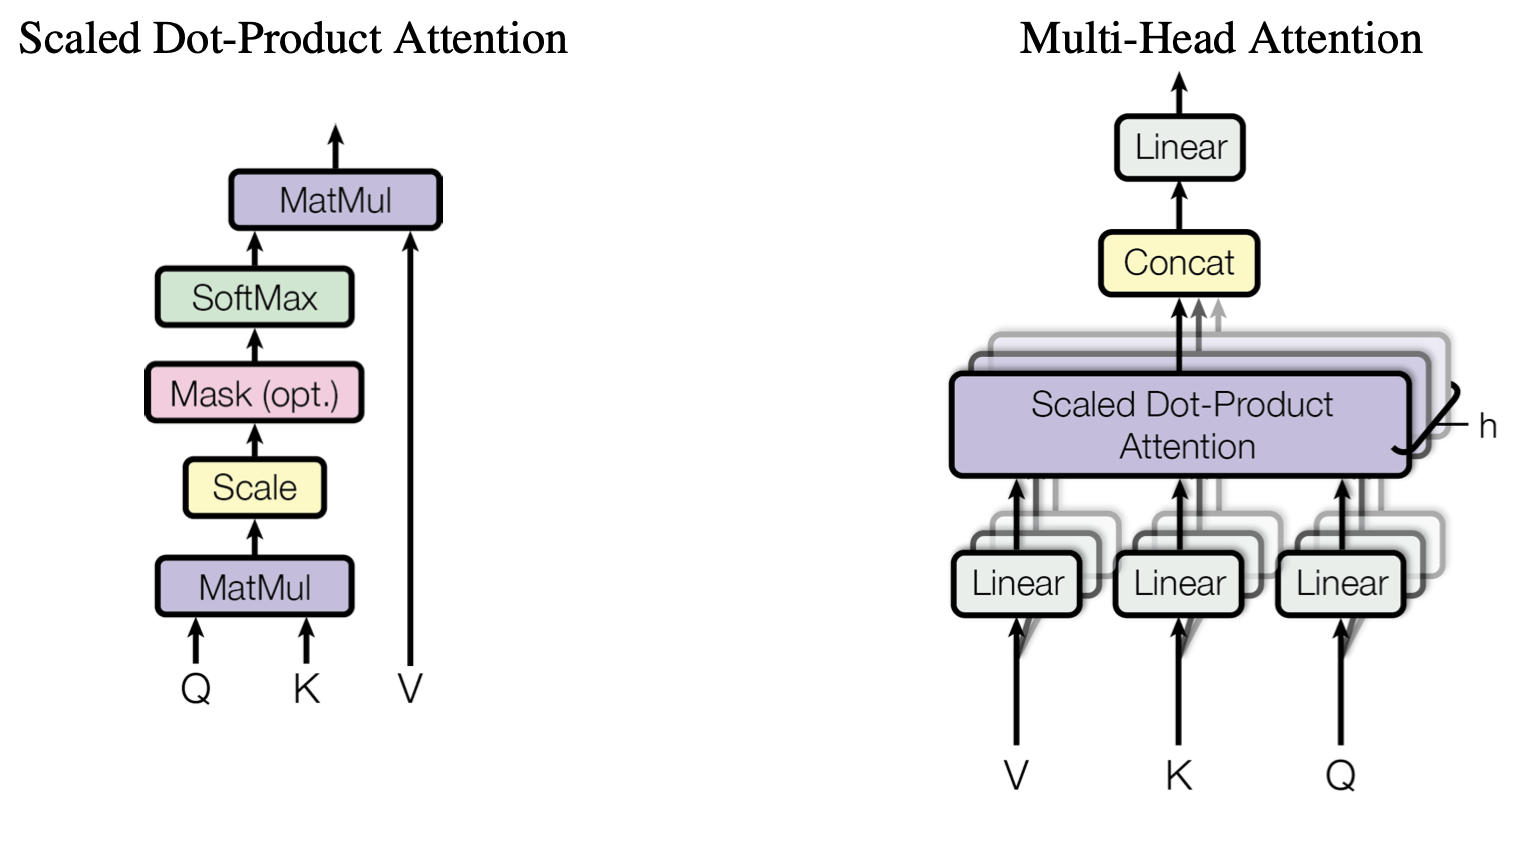
\includegraphics[width = 1\linewidth]{figures/Attention.png}
\caption{(left) Scaled Dot-Product Attention. (right) Multi-Head Attention. Figure obtained from \citet{vaswani2017attention}.}
\label{fig:attention}
\end{figure}

This is the so-called \textit{scaled dot-product attention}. Whereas \citet{vaswani2017attention} use so-called \textit{multi-head attention} to build transformers. Rather than calculating a single attention, they split $Q, K$ and $V$ into $h$ vectors and apply self-attention to each of them. This means that the model has $h$ different heads, each of which should learn something different. This is supposed to give the model more representation power. The different heads are computed in parallel and concatenated at the end. The final values are obtained by linearly projecting the concatenated values. Both scaled dot-product and multi-head attention are visualized in Figure \ref{fig:attention}.

This encoder-decoder architecture is the second important concept needed to understand transformers. Introduced in \citet{sutskever2014sequence} this architecture is used in many NLP models including transformers. It is used to deal with the problem of in- and output sequences being of different lengths. Imagine, for example, the simple task of translating from one language to another. It will often be the case that the translation does not have the same number of sentences/words/characters as the input. That is where the encoder-decoder comes into play. First, the encoder model transforms the input into a vector of a fixed size. This vector is supposed to contain all of the information from the input. A second model, the decoder, then takes this vector as an input and predicts the outcome. As a result the input and the output sequences don't have to be of the same lengths. 

\begin{figure}[h!]
\centering
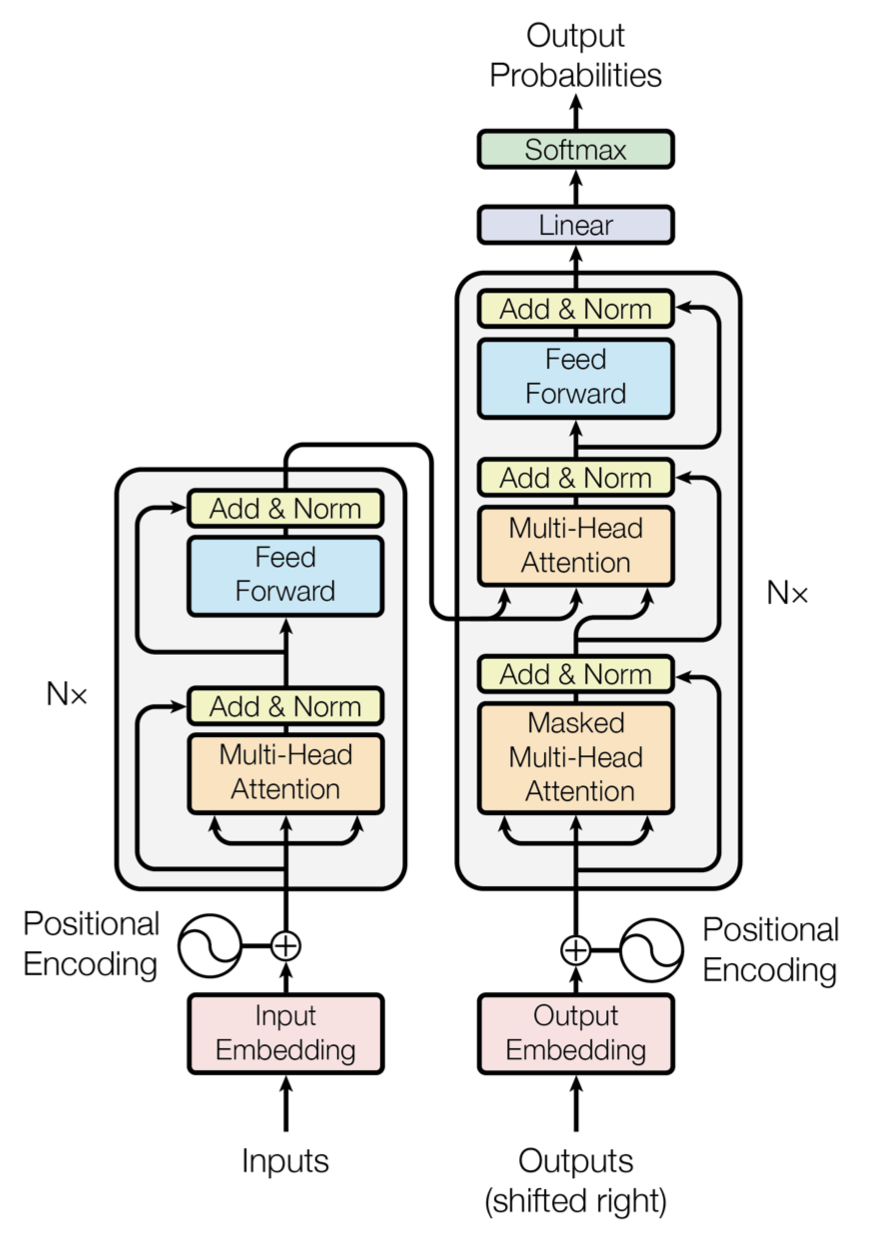
\includegraphics[width = 10cm]{figures/Transformer.png}
\caption{Transformer-model architecture. Figure obtained from \citet{vaswani2017attention}.}
\label{fig:transformer}
\end{figure}

Putting those two ideas together leads to the final transformer architecture, as shown in Figure \ref{fig:transformer}. The basic idea behind each step will now be briefly explained, starting with the encoder. As explained previously, the encoder is used to map the input sequences into continuous representations that hold all of the learned information from the input together with context added through attention that will help the decoder focus on the important tokens.

Since NNs can only deal with numerical input and not with text, the texts must be converted. First they are tokenized, i.e. divided into individual words or meaningful sub-words. These tokens are then transformed into embeddings, i.e. numerical vectors that are representations of the text input. The absence of recurrence or convolution in the model would cause it to loose information on the sequence's order. That is why the next step is to inject positional information into the embeddings. \citet{vaswani2017attention} do this using sine and cosine functions, creating vectors depending on the time step, and adding those vectors to the embeddings.

Next comes the encoder layer (\citet{vaswani2017attention} use a stack of $N=6$ identical layers). It starts with multi-head self-attention. Self-attention is a special type of attention that allows the model to relate each token in the input sequence to the other tokens in that sequence. This is done so the model knows which tokens to pay attention to when dealing with a certain token. There is a residual connection \citep{he2016deep} around the multi-head self-attention, followed by a normalization \citep{ba2016layer}. That means that the output from the multi-head attention gets added to the embeddings (with positional encoding), and together they are normalized. This then gets fed into a point-wise feed-forward NN consisting of two linear layers with a ReLU activation \citep{nair2010rectified} in between them. There is also a residual connection around, which gets added to the output of the feed-forward network and is normalized.

Next is the decoder. \citet{vaswani2017attention} stack $N=6$ identical layers. Each consists of three sub-layers, each with a residual connection around it, followed by layer normalization. The decoder gets two inputs: the true outputs (what it should predict) and the output from the encoder. Before being fed into the decoder, the true outputs are being embedded and positional encodings are added analogous to to the inputs for the encoder. Next, a masked multi-headed self-attention layer is applied. Future tokens shouldn't be taken into account by the decoder since it creates a sequence token by token and is autoregressive. That is why this attention layer is masked, a mask (setting attentions to $-\infty$) is placed on future tokens to prevent them from influencing predictions. This mask is added to the score matrix before scaling it, which leads the attention scores for future tokens to be zero and the model essentially ignoring those tokens. Apart from the masking, the process is the same as for the multi-headed self-attention layer in the encoder.

Next is the multi-head ``encoder-decoder attention''. The output of the encoder serves as the source for the keys and values, while the queries are derived from the preceding decoder layer. Therefore, each location in the decoder can pay attention to every position in the input sequence, allowing the decoder to decide which encoder input is important. The feed-forward layer is built in the same way as in the encoder. Finally, the output goes through a linear layer that acts as a classifier, and after softmax is applied, it outputs the probabilities between 0 and 1 for each token.

By demonstrating that self-attention could be used instead of recurrent and convolutional neural network architectures, the transformer architecture revolutionized the field of NLP. LMs' accuracy and speed both significantly increased as a result of this innovation, enabling state-of-the-art performance on a variety of language tasks. Some of the most cutting-edge LMs to date, including GPT-3 \citep{brown2020gpt3} and BERT \citep{devlin2018bert}, were created using the transformer architecture, which has come to be the de facto standard for many applications of NLP.

\section{Pre-trained Language Models}\label{models}

Pre-training is a widely used technique for NLP transfer learning tasks that involves training a large LM on tons of text data before fine-tuning it for a particular task. Pre-training aims to learn a rich representation of a language's underlying linguistic relationships and patterns. The model can then be fine-tuned using this representation as a strong starting point to perform a specific task, such as political stance prediction.

Using a pre-trained model offers several benefits over training a model from scratch. The large amounts of text data used have already taught the Pre-trained model a lot of information that can be used to boost performance on the target task. When compared to training a model from scratch, this can save time and computational resources while also improving overall performance.

In recent years, several pre-trained LMs have been introduced that have shown remarkable performance on a range of language tasks. ELMo \citep{peters2018elmo}, BERT \citep{devlin2018bert}, T5 \citep{xue2020mt5}, ELECTRA \citep{clark2020electra}, and various GPT models \citep{radford2018gpt, radford2019language, brown2020gpt3} are some examples of these models. Following is a brief introduction to each of the different models, followed by some solutions on how to use them when handling non-English (specifically German) text data.

\subsection{ELMo} \label{elmo}

\citet{peters2018elmo} introduce ELMo (\textbf{E}mbeddings from \textbf{L}anguage \textbf{Mo}dels), a bidirectional LM that combines a forward and a backward LM. Bidirectional means that the model can use information from both sides (what happened before and after the current token). ELMo uses two BiLSTMs, which consist of two separate unidirectional LSTMs, to achieve its bidirectionality. This is not only a ``shallow'' concatenation of independently trained unidirectional LMs \citep{devlin2018bert}, but the sequential nature of the LSTMs means that ELMo a) is not fully parallelizable and b) fails to capture long-range dependencies during contextualization.


\subsection{GPT models} \label{gpt}

OpenAI created a group of deep learning models known as the GPT (\textbf{G}enerative \textbf{P}re-trained \textbf{T}ransformer) model family. The first model in the series, GPT-1, was introduced in June 2018 \citep{radford2018gpt} and was followed by GPT-2, GPT-3 and ChatGPT \citep{radford2019language, brown2020gpt3, chatgpt}.

GPT-1 \citep{radford2018gpt} is a transformer that combines multiple decoder blocks with a standard LM objective for pre-training and can then be fine-tuned with task-specific data. The architecture supported transfer learning and could carry out a variety of NLP tasks with little tweaking. GPT-1 demonstrated the value of pre-training a model and then adapting the fine-tuning depending on the task, which improves the model's generalization. The model provided a starting point for other models that could more fully realize this potential with larger datasets and more parameters. But while GPT-1 solved some of the problems of previously released ELMo, it is still just unidirectionally contextual.

Using a larger dataset and adding more parameters to the model were the main developments in the GPT-2 model that was introduced a year later \citep{radford2019language}. But there were also some other changes. The goal of GPT-2 was to learn multiple, different tasks using the same unsupervised model. This is called task conditioning, the model is supposed to produce a different output for the same input if given a different task. In order to condition a LM on a task, examples or plain-language instructions are given to the model. Being able to task condition makes GPT-2 capable of zero-shot learning and zero-shot task transfer. Zero-shot learning refers to the ability of a model to recognize and classify objects or concepts it has never seen before. Zero-shot task transfer means that the model is able to perform a task without being specifically trained on it. The input was formatted so that the model had to comprehend the task at hand and respond appropriately. For instance, in a question-answering task, the input would be the question followed by a question mark (?), indicating that the model was expected to generate an answer. Without any prior experience with that specific task, the model was created to understand the nature of the task and provide accurate answers.

Open AI developed the GPT-3 \citep{brown2020gpt3} model with 175 billion parameters, which has 100 times more parameters than GPT-2, in an effort to create an extremely robust and powerful LM that would require little to no fine-tuning and only a few demonstrations to comprehend tasks and carry them out. GPT-3 is trained to be capable of zero-shot and few-shot learning. Few-shot learning refers to the ability to perform a task with only a few examples. This means that users can provide a few examples and a description of the task, and the model can use this information to generate new outputs. In addition to growing in size and getting better at learning, GPT-3 has a wider range of tasks it can complete. This includes coding, summarizing, translating languages, and answering questions. The model can produce realistic text in a range of genres and styles, making it useful even for literary or artistic endeavors like writing poetry or fiction.

ChatGPT \citep{chatgpt} is a web app to generate natural language texts for chatbot applications. Due to its specialized optimization for dialogue, which enables it to carry out tasks like explaining code or writing poems in a more chat-like manner, and its accessibility to the public it quickly rose to popularity. With 20 billion parameters, ChatGPT has been specifically designed to generate human-like text in the context of chatbot conversations and has been trained with specific datasets of chatbot interactions.


\subsection{BERT} \label{bert}

BERT stands for \textbf{B}idirectional \textbf{E}ncoder \textbf{R}epresentations from \textbf{T}ransformers and was proposed to solve these existing problems. Introduced by \citet{devlin2018bert}, it completely replaces recurrent architectures with self-attention by using multiple transformer encoder blocks. The unidirectionality constraint is alleviated by pre-training using a Masked Language Model (MLM) objective.

\citet{devlin2018bert} reports results on two models: $BERT_{BASE}$ and $BERT_{LARGE}$ which have the same general architecture and training steps but differ in size. $BERT_{BASE}$ has 12 layers (transformer blocks), a hidden size of 768, and 12 self-attention heads, while $BERT_{LARGE}$ has 24 layers, a hidden size of 1024, and 16 self-attention heads.

BERTs training can be divided into two steps: pre-training and fine-tuning. During pre-training, the model is trained on unlabeled data over two tasks. The first task is the already mentioned MLM. 15\% of the tokens are masked at random using [MASK] tokens, and the model is then trained to predict those masked tokens. This makes BERT bidirectional but at the same time solves the problem of standard bidirectional conditional models where each word indirectly ``sees itself'' \citep{devlin2018bert}.

The second task is Next Sentence Prediction (NSP). As an input, they use two sentences. 50\% of the time, they actually follow each other in the training data, and the other half is just two random sentences from the corpus. The model is trained to detect if the second sentence follows the first. This allows the model to learn the relationship between two sentences.

The pre-trained model has a general understanding of language and then gets fine-tuned depending on the task it is supposed to complete. This is a simple matter of just using task-specific in- and outputs. The input could, for example, be a hypothesis-premise pair that should be classified as true or false. To get the output, the token representing the sequence ([CLS]) is fed into a classification layer. The model then gets initialized with the parameters learned from pre-training and fine-tunes them while training on this (new) downstream task. Since not a whole new model has to be trained, this makes fine-tuning BERT relatively inexpensive and also applicable to a lot of different tasks.

\subsection{ELECTRA} \label{electra}

The name ELECTRA stands for \textbf{E}fficiently \textbf{L}earning an \textbf{E}ncoder that \textbf{C}lassifies \textbf{T}oken \textbf{R}eplacements \textbf{A}ccurately. The model was introduced by \citet{clark2020electra}. Unlike BERT, ELECTRA learns from all of the tokens, which is due to a different pre-training objective. It replaces the old MLM task with a new task called Replaced Token Detection (RTD). Additionally, ELECTRA makes use of a novel generator-discriminator architecture that is inspired by the GAN (Generative Adversarial Network) framework used in computer vision.

\begin{figure}[h!]
\centering
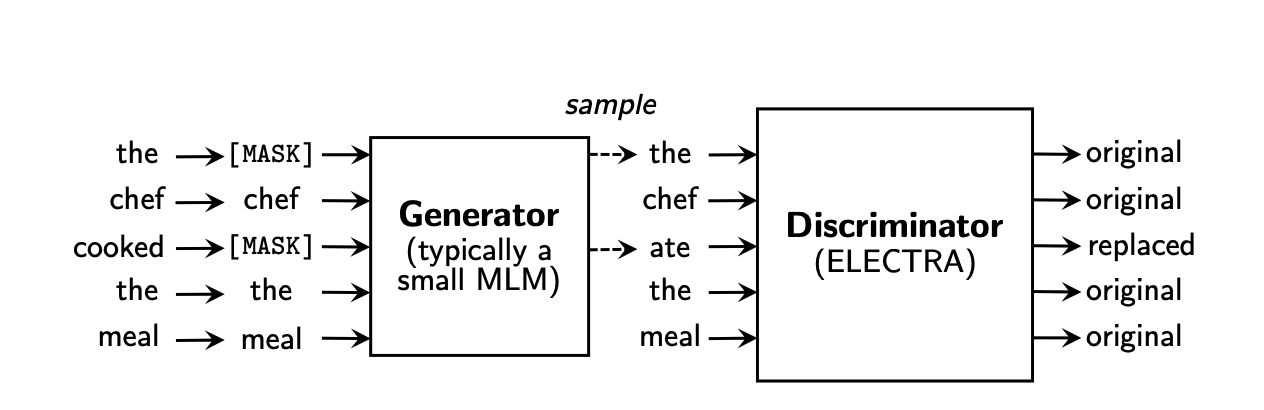
\includegraphics[width = 1\linewidth]{figures/electra.png}
\caption{Generator-Discriminator Architecture used for ELECTRA. Figure obtained from \citet{clark2020electra}.}
\label{fig:electra}
\end{figure}

The generator is an encoder that learns to replace [MASK] tokens (this is a typical MLM objective). The discriminator network then predicts whether each token in the sequence is original (real) or replaced by the generator (fake). This is the novel RTD task. Instead of just predicting the original masked token, the model learns to predict whether a token in a sequence has been replaced by a fake token. This pre-training objective is more compute-efficient than MLM and results in improved performance on subsequent tasks \citep{clark2020electra}.

\citet{clark2020electra} have demonstrated that this new pre-training task is effective. Because RTD defines the task over all input tokens rather than just a select few that are masked out, it is found to be more efficient than MLM. Given the same model size, data, and compute, the contextual representations learned by ELECTRA perform better than those learned by BERT.


\subsection{T5} \label{t5}

The T5 model is a text-to-text transfer learning framework based on transformers that can carry out a variety of NLP tasks, such as question answering, summarizing, and translation, among others. It was first introduced by \citet{raffel2020exploring}. T5 employs a unified architecture as opposed to earlier models, allowing it to be trained on various tasks just by altering the prefix added to the input sequence. With this method, the model can handle multiple tasks with a single architecture.

The model itself is similar to the original transformer proposed by \citet{vaswani2017attention} but removes the layer norm bias, places the layer normalization outside the residual path, and uses a different position embedding scheme \citep{raffel2020exploring}. In contrast to models like BERT or ELECTRA, T5 is a ``text-to-text'' model, which means that it has been trained to map input text sequences to output text sequences. As opposed to many other NLP models, which are trained for particular tasks like classification, translation, or question-answering, this makes T5 general-purpose. In order to be able to carry out the different tasks, T5 employs a ``task prefix'', which identifies the precise task being carried out, enabling the model to be more precisely tuned for a particular task (more on this in section \ref{task_prefix}). Figure \ref{fig:t5} shows how the task prefixes work together with the text-to-text framework.

\begin{figure}[h!]
\centering
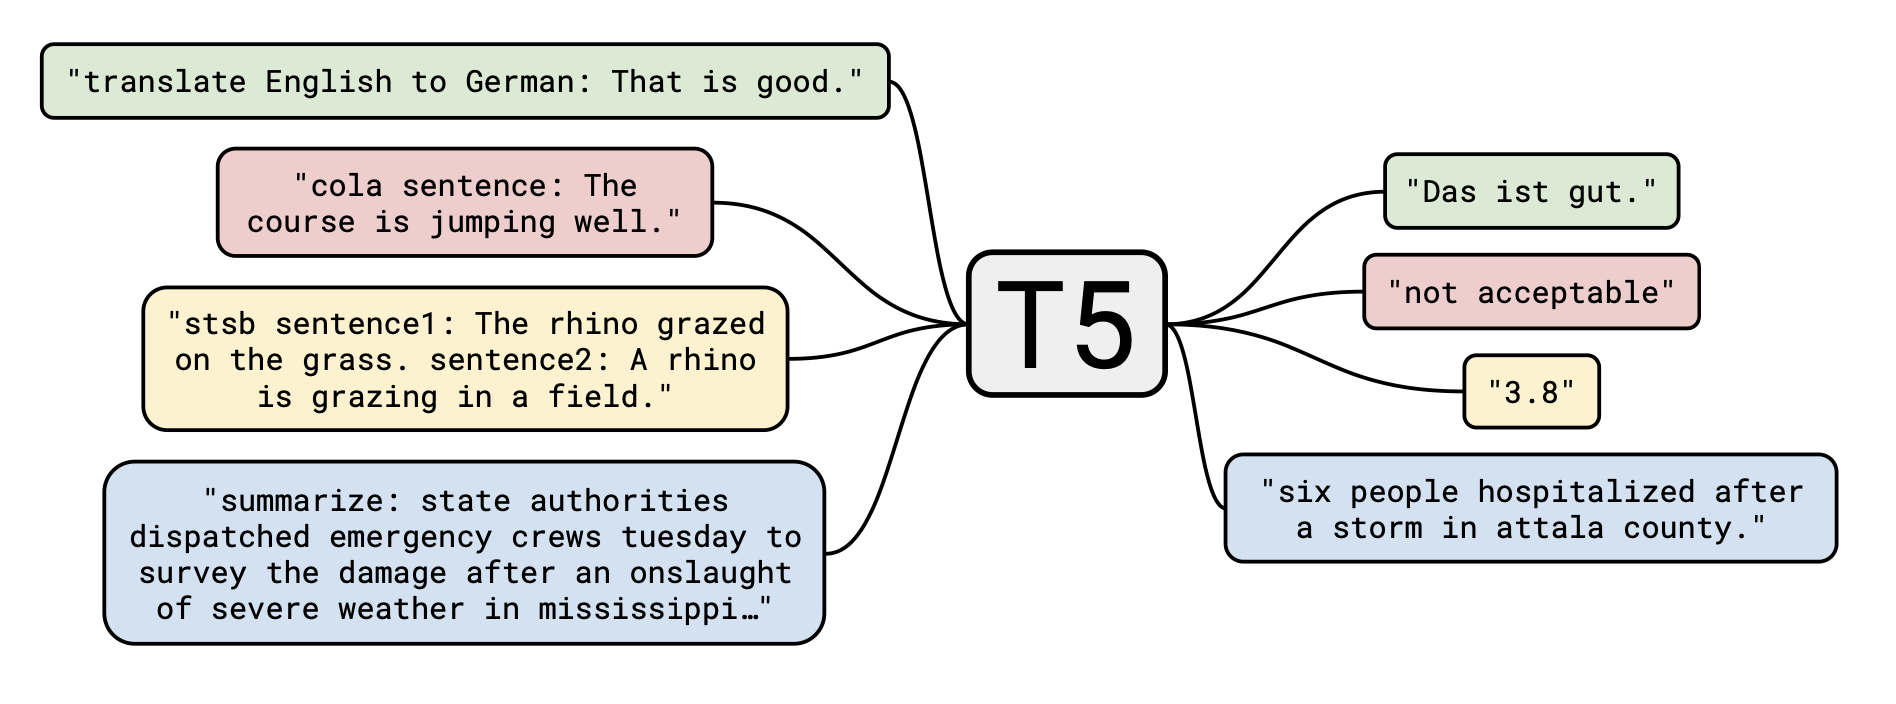
\includegraphics[width = 1\linewidth]{figures/t5.png}
\caption{Examples how the T5 text-to-text framework with task prefixes works. Figure obtained from \citet{raffel2020exploring}.}
\label{fig:t5}
\end{figure}

As \citet{roberts_2020} explains, the pre-training objective is to predict missing words in a corrupted text. These ``blanks'' can also appear at the end of the text, making this objective a generalization of a continuation task. They developed a new downstream task called ``sized fill-in-the-blank'', which asks the model to fill in a blank with a predetermined number of words. One could train the model to fill in the blank with roughly two words by giving it the input ``I like to eat peanut butter and \underline{\hspace{2mm}}2\underline{\hspace{2mm}} sandwiches.'' for instance. The model would then predict something like ``I love peanut butter and jelly on my sandwiches.'', filling the blank with three words.

The authors train five variants of T5: a small model, a base model, a large model, and models with 3 billion and 11 billion parameters. They perform well overall, with the exception of translation. The fact that they are able to perform nearly as well as humans on the SuperGLUE natural language understanding benchmark — which is made specifically to be challenging for machine learning models but simple for humans — is one of their more impressive results.


\subsection{German Models} \label{german_models}

NLP has undergone a revolution thanks to the creation of LMs like the ones discussed, which have allowed researchers and practitioners to create more precise and effective algorithms for a variety of tasks. These models, however, are not applicable to other languages than the ones they were trained on (most of the time English), necessitating the development of language-specific models to guarantee the best results on tasks involving a given language. In order to deal with the data presented in this thesis, models that are able to deal with the German language are needed.

There are two approaches to this. Either train an architecture from scratch with German data or use a model that is capable of understanding multiple languages (including German). For ELMo, BERT and ELECTRA the first approach was chosen. \citet{GerElmo} train a German ELMo on the German Wikipedia Text Corpus.

There are several German BERT models available that use the BERT architecture but have been trained on large German language corpora. For the following experiments, ``bert-base-german-cased'' is used. It was trained by \citet{german_bert} on German news articles, German Wikipedia, and open legal data (German court decisions). 

Instead of the English ELECTRA, this thesis uses the German ``electra-base-german-uncased'' \citep{german_electra}. Trained on the Cleaned Common Crawl Corpus 2019-09 German, German Wikipedia, Subtitles, and News, this model is the top-performing publicly available German NLP model on a variety of German evaluation metrics.

GPT-3 is multilingual right out-of-the-box and can produce text in a wide range of languages, including English, Spanish, French, German, Chinese, and many others, because it was trained on an extensive set of text from the internet. It is important to remember that the performance of the model will differ depending on the language and level of complexity of the text being generated. Additionally, mGPT \citep{shliazhko2022mgpt}, a model that supports 60 languages, is available.

For T5, there is also a multilingual model. mT5 \citep{xue2020mt5} is the multilingual version of T5 and was pre-trained on a corpus covering 101 languages, including German. Unlike T5, it has to be fine-tuned before it is usable on a downstream task.


\section{Semantic Search}\label{semantic_search}

In order to find relevant information from a text (in this case, the party manifestos), one has to employ a search. When given a query sentence, the goal is to find the sentences in the text that are the most related to the query.

Semantic search is one of the techniques that could be used and refers to the process of finding information in a more human-like way by taking into account the meaning of the search query and the context in which it is being made. Traditional keyword-based search techniques (like BM25) only match the exact terms that the user enters, but semantic search goes beyond this. Semantic search seeks to comprehend the purpose of the query and the relationships between the words in order to provide more accurate results.

Word, sentence, or paragraph embeddings are the key component used in semantic search. Embeddings are numerical representations of words that capture the meaning and context of words in a continuous vector space. These representations enable word (or sentence or paragraph) comparison based on similarity and are learned using different algorithms (some of which will be presented here).

A central concept in semantic search is similarity. It measures how close two words or phrases are to each other in meaning. One way to determine the similarity between the phrase embeddings of the search query and the documents being searched is by calculating the dot products. The higher the product, the more likely it is that the sentence is relevant to the query.

In the following chapter, different approaches to semantic search (and BM25 as a baseline) are described. And later on (in Chapter \ref{results}), the results are compared, giving an estimate of how well they work together with the different models.


\subsection{BM25} \label{bm25}

BM25 is a ranking function to determine the relevance of documents to a given query, often used by search engines. It was developed in the mid-1990s by Stephen E. Robertson, Karen Spärck Jones, and others \citep{robertson1995okapi}. It utilizes a bag-of-words retrieval function. A set of documents is ranked based on the number of query terms appearing in each of the documents. There are multiple implementations; here, BM25+, as introduced by \citet{lv2011lower}, is used. It is chosen over other adaptations since, first of all, it shows good performance in \citet{trotman2014rankbm25}, and second, it is implemented in the python package \textit{rank\_bm25} by \citet{rank_bm25}.

The retrieval status value $rsv_q$ for a given query $q$ is computed as follows:

\begin{equation}
    rsv_q = \sum_{t \in q} log \left( \frac{N+1}{df_t} \right) \cdot \left( \frac{(k_1 + 1) \cdot tf_{td}}{k_1 \cdot \left( (1-b)+b \cdot \left( \frac{L_d}{L_{avg}}\right) \right) +tf_{td}} + \delta \right),
\end{equation}

where $q$ is the query with individual terms $t$. $N$ is the number of documents in the collection, $df_t$ is the document frequency (the number of documents containing the term $t$), $tf_{td}$ is the number of times a term occurs in document $d$. $L_d$ is the length of the document (in terms), and $L_{avg}$ is the average document length. $k_1, b$ and $\delta$ are parameters to be tuned.

BM25 (and all the different adaptations) is, in contrast to the other methods that follow, a simple keyword-based algorithm and has nothing to do with BERT or other LMs. It is chosen as a baseline to compare the much more complicated semantic search methods to.


\subsection{SBERT}\label{sbert}

Earlier, BERT was introduced as a model for NLP. However, it is not suitable for semantic similarity search. To compute the similarity between a group of sentences, all pairs of sentences have to be fed into the network. That means that for a collection of 10 000 sentences, BERT has to do 49 995 000 pairwise computations \citep{reimers2019sbert}. This is often solved by obtaining fixed-size embeddings for the sentences, either by averaging the BERT output layer or by using the output of the [CLS] token (which appears at the beginning of every sentence). But as \citet{reimers2019sbert} show, this practice doesn’t produce good sentence embeddings.
Instead, they offer a modification of BERT called SBERT (Sentence-BERT), which fine-tunes BERT. By using siamese and triplet networks, they update the weights in such a way that the produced sentence embeddings are semantically meaningful while still maintaining the accuracy of the original BERT. The result are fixed-size embedding vectors for input sentences that can be compared with each other using similarity measures like cosine-similarity or dot product.

The network structure that has to be trained depends on the data at hand. \citet{reimers2019sbert} present three objective functions to deal with sentence embeddings obtained from BERT (they also experiment with ways to obtain the embeddings, for more on that, please see the paper):
\begin{itemize}
    \item \textit{Classification Objective Function} (visualized in Figure \ref{fig:sbert}):
    The two sentence embeddings, $u$ and $v$ are concatenated with the element-wise difference $|u-v|$ and multiplied with a trainable weight $W_t$. Then a softmax is applied. The objective function is optimized using cross-entropy loss.
    \begin{equation}
    o=\text{softmax}(W_t (u,v,|u-v|))
    \end{equation}
    \item \textit{Regression Objective Function}:
    The cosine-similarity between $u$ and $v$ is computed, and mean-squared-error loss is used as the objective function.
    \item \textit{Triplet Objective Function}:
    Instead of pairs, there are now triplets of sentences, an anchor sentence with embedding $a$, a positive sentence with embedding $p$ and a negative sentence with embedding $n$. The goal is to get a smaller distance between $a$ and $p$ than between $a$ and $n$. This can be achieved by minimizing the following loss function:
    \begin{equation}
    max(||a-p||-||a-n||+\epsilon,0)
    \end{equation}
    where $||\cdot||$ is Euclidean distance and margin $\epsilon = 1$.
\end{itemize}

\begin{figure}[h!]
\centering
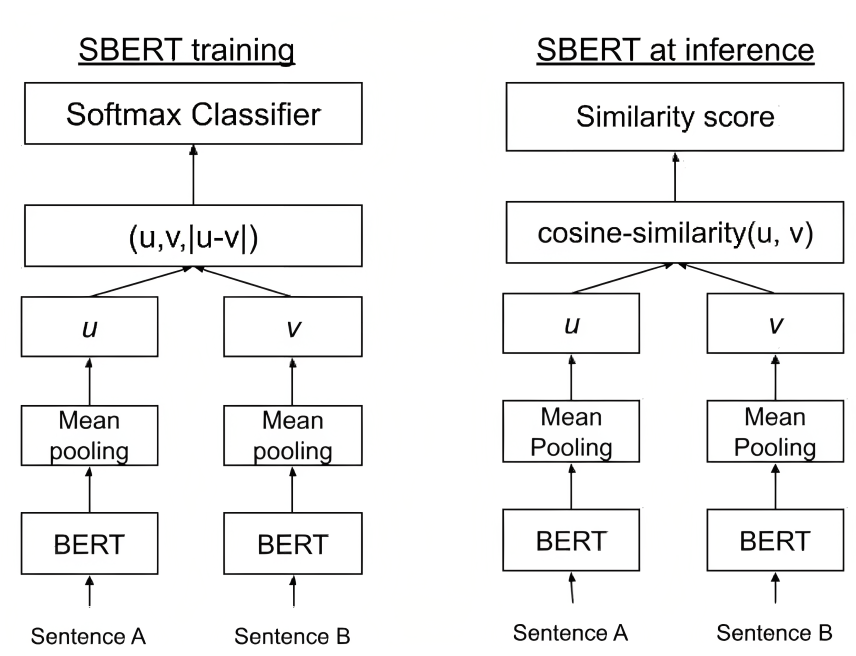
\includegraphics[width = 0.8\linewidth]{figures/SBERT.png}
\caption{Illustration of the Classification Objective Function of SBERT. Figure obtained from \citet{sbert}.}
\label{fig:sbert}
\end{figure}

It is important to remember that training a SBERT model requires labeled sentence pairs. There are, however, a variety of pre-trained models that can be used to produce high-quality embeddings for numerous downstream tasks without the need for those labeled pairs. Since the data for this thesis doesn't contain labeled sentence pairs, ``paraphrase-multilingual-mpnet-base-v2'' \citep{reimers2019sbert}, one of those pre-trained models that supports German, is used.

\subsection{BERT-Flow}\label{bert-flow}

\citet{li2020bertflow} follow a different approach. They attribute the poor performance of BERT sentence embeddings (obtained by mean pooling over the first and last layers) to not fully exploiting the semantic information that already exists in the BERT embeddings. BERT's sentences live in a non-smooth, anisotropic semantic space, which hinders semantic similarity tasks. That is why they propose an unsupervised approach to transform the embedding distribution. Through normalizing flows, the anisotropic, non-smooth distribution is changed to a smooth and isotropic Gaussian distribution, as is illustrated in Figure \ref{fig:bert_flow}. By using an invertible mapping from the BERT embedding space to the Gaussian space, the information encoded in the embeddings does not change, but the embeddings are better at semantic similarity tasks. To achieve this \citet{li2020bertflow} ``learn a flow-based generative model by maximizing the likelihood of generating BERT sentence embeddings from a standard Gaussian latent variable''.

\begin{figure}[h!]
\centering
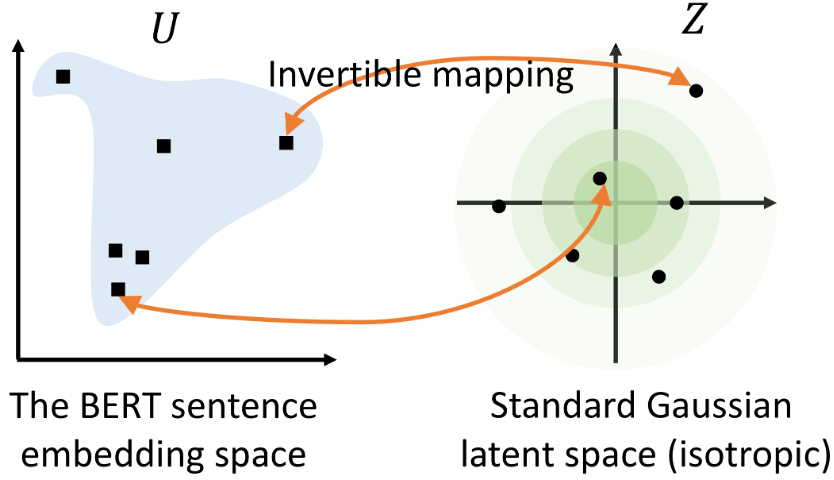
\includegraphics[width = 0.8\linewidth]{figures/BERT-Flow.png}
\caption{Illustration of the goal of BERT-Flow. Figure obtained from \citet{li2020bertflow}.}
\label{fig:bert_flow}
\end{figure}

They call the observed space (the BERT embedding space) $U$, and the latent space (the standard Gaussian latent space) $Z$. The goal is to learn $f: Z \to U$ with $u=f_\phi (z)$, which is an invertible transformation. $z \sim p_Z (z)$ is the prior distribution, a standard Gaussian distribution. The probabilistic density function for $U$ is given as

\begin{equation}
    p_U (u)=p_Z (f^{-1}_\phi (u)) |det \frac{\partial f^{-1}_\phi (u)}{\partial u}|.
\end{equation}

Therefore, in order to maximize the likelihood of $U$'s marginal solve

\begin{equation}
    max_\phi \quad \mathbb{E}_{u=BERT(sentence), sentence \sim D} \quad log(p_Z (f^{-1}_\phi (u))) + log(|det \frac{\partial f^{-1}_\phi (u)}{\partial u}|)
\end{equation}

where $D$ denotes the dataset.

Using the learned function $f_\phi$ and inverting it makes it possible to transform all BERT sentence embeddings $u$ into latent standard Gaussian representations $z$. \citet{li2020bertflow} follow an approach similar to Glow \citep{kingma2018glow} by stacking multiple invertible transformations to parameterize $f_\phi$ as a neural network. It is important to note that training only affects the parameters of $f_\phi$ while the BERT parameters remain unchanged. Additionally, this implies that BERT-Flow can be used with any sentence embeddings. Both BERT (mean pooling over the first and last layers) and SBERT embeddings are used in this thesis.

\subsection{Whitening}\label{whitening}

Whitening also attempts to solve the problem of non-smooth, anisotropic distribution. But instead of learning a network like with BERT-Flow, \citet{huang2021whiteningbert} use a simple linear transformation. Whitening normalizes sentence embeddings with the goal of improving semantic similarity matching. It does this by transforming the covariance matrix to an identity matrix using a given mean and covariance matrix. The mean and covariance matrices are estimated from the sentence embeddings $D$ (obtained by mean pooling the BERT embeddings). By applying

\begin{equation}
    \hat{D}=(D-\mu)OC^{-\frac{1}{2}}
\end{equation}

where $\mu$ is the mean vector of $D$, $C$ is a diagonal matrix with the eigenvalues of the covariance matrix $Cov(D)=(D-\mu)^T(D-\mu)$ and $O$ is the corresponding orthogonal matrix of eigenvectors (satisfying $Cov(D)=OCO^T$), one gets the whitened sentence embeddings $\hat{D}$.
This approach is much simpler and easier to implement since it only requires estimating $\mu$ and $C$, while BERT-Flow calls for a whole NN to be trained. As the process of Whitening can be applied to any sentence embeddings, it is utilized in this thesis on BERT (mean pooling) and SBERT embeddings.

\subsection{SBERT-WK}\label{sbert-wk}

\citet{wang2020sbertwk} propose a method of dissecting BERT-based models through geometric analysis of the space spanned by the word representations. The goal is to make use of all the different layers of BERT that capture different linguistic properties. SBERT-WK doesn't require further training; it uses existing word representations and adds them together in a new way to form a sentence embedding.

The first step is to look at each word's alignment and novelty properties, and then combine the word's representations across layers to construct a unified word representation. To then get the final sentence embedding vector, a weighted average of all unified word representations is computed based on the word importance measure.

To compute the unified word representation $\hat{v}_w$ of word $w$ (for all $N$ words) \citet{wang2020sbertwk} assign weight $\alpha_i$ to the words $i$-th layer representation $v^i_w$ and take an average:

\begin{equation}
    \hat{v}_w = \sum_{i=0}^{N} \alpha (v^i_w) v^i_w.
\end{equation}

The weights $\alpha$ are a weighted average of two ways to measure the new information brought by a word interpretation at the $i$-th layer: inverse alignment and novelty. For a more detailed explanation of the two see the paper \citep{wang2020sbertwk}. The idea behind the inverse alignment measure is that if neighboring layers word representations align well, they don't provide much additional information, so the weight should be small. Therefore, the inverse of the alignment similarity score is used. Novelty measures the new information a word representation brings with respect to the subspace spanned words in its neighboring window. Using a weighted average of those two measures finally leads to a unified word representation for each word.

In the next step, the unified word representations get added together to form a sentence embedding $v_s$

\begin{equation}
    v_s = \sum_{j} \omega_j \hat{v}_{w(j)}
\end{equation}

where $\hat{v}_{w(j)}$ is the unified word representation for the $j$-th word in a sentence.

They are weighted by their importance $\omega_j$, which is defined as

\begin{equation}
    \omega_j = \frac{|\sigma^2_j|}{\sum_{k} |\sigma^2_k|},
\end{equation}

where $\sigma^2_j$ is the variance of the offset-1 diagonal values of the cosine similarity matrix for the $j$-th word. That means that words that develop more quickly across layers get higher weights.

\subsection{IS-BERT}\label{is-bert}

IS-BERT is an extension on top of BERT that can learn sentence representations in an unsupervised manner, as proposed by \citet{zhang2020isbert}. As mentioned before, sentence embeddings for BERT are often obtained by averaging the BERT output layer or by using the output of the [CLS] token. Instead, IS-BERT uses CNN (Convolutional Neural Network) layers with mean-over-time pooling, which are trained using a novel self-supervised objective that maximizes the mutual information between the global sentence embeddings and all of their local context embeddings. In order to utilize all the aspects of a sentence's local context information, the local contexts of other sentences are used as negative examples for contrastive learning.

In general, contrastive learning is a machine learning approach used to learn the general characteristics of a dataset without the need for labels by teaching the model to differentiate between similar and different data points. Instead of labels, the model needs pairs. A positive pair consists of two similar data points, and a negative pair consists of two contrasting data points. The model computes a similarity measure for the pairs and gets trained in such a way that the similarity for positive pairs should be high and that for negative pairs should be low.

\begin{figure}[h!]
\centering
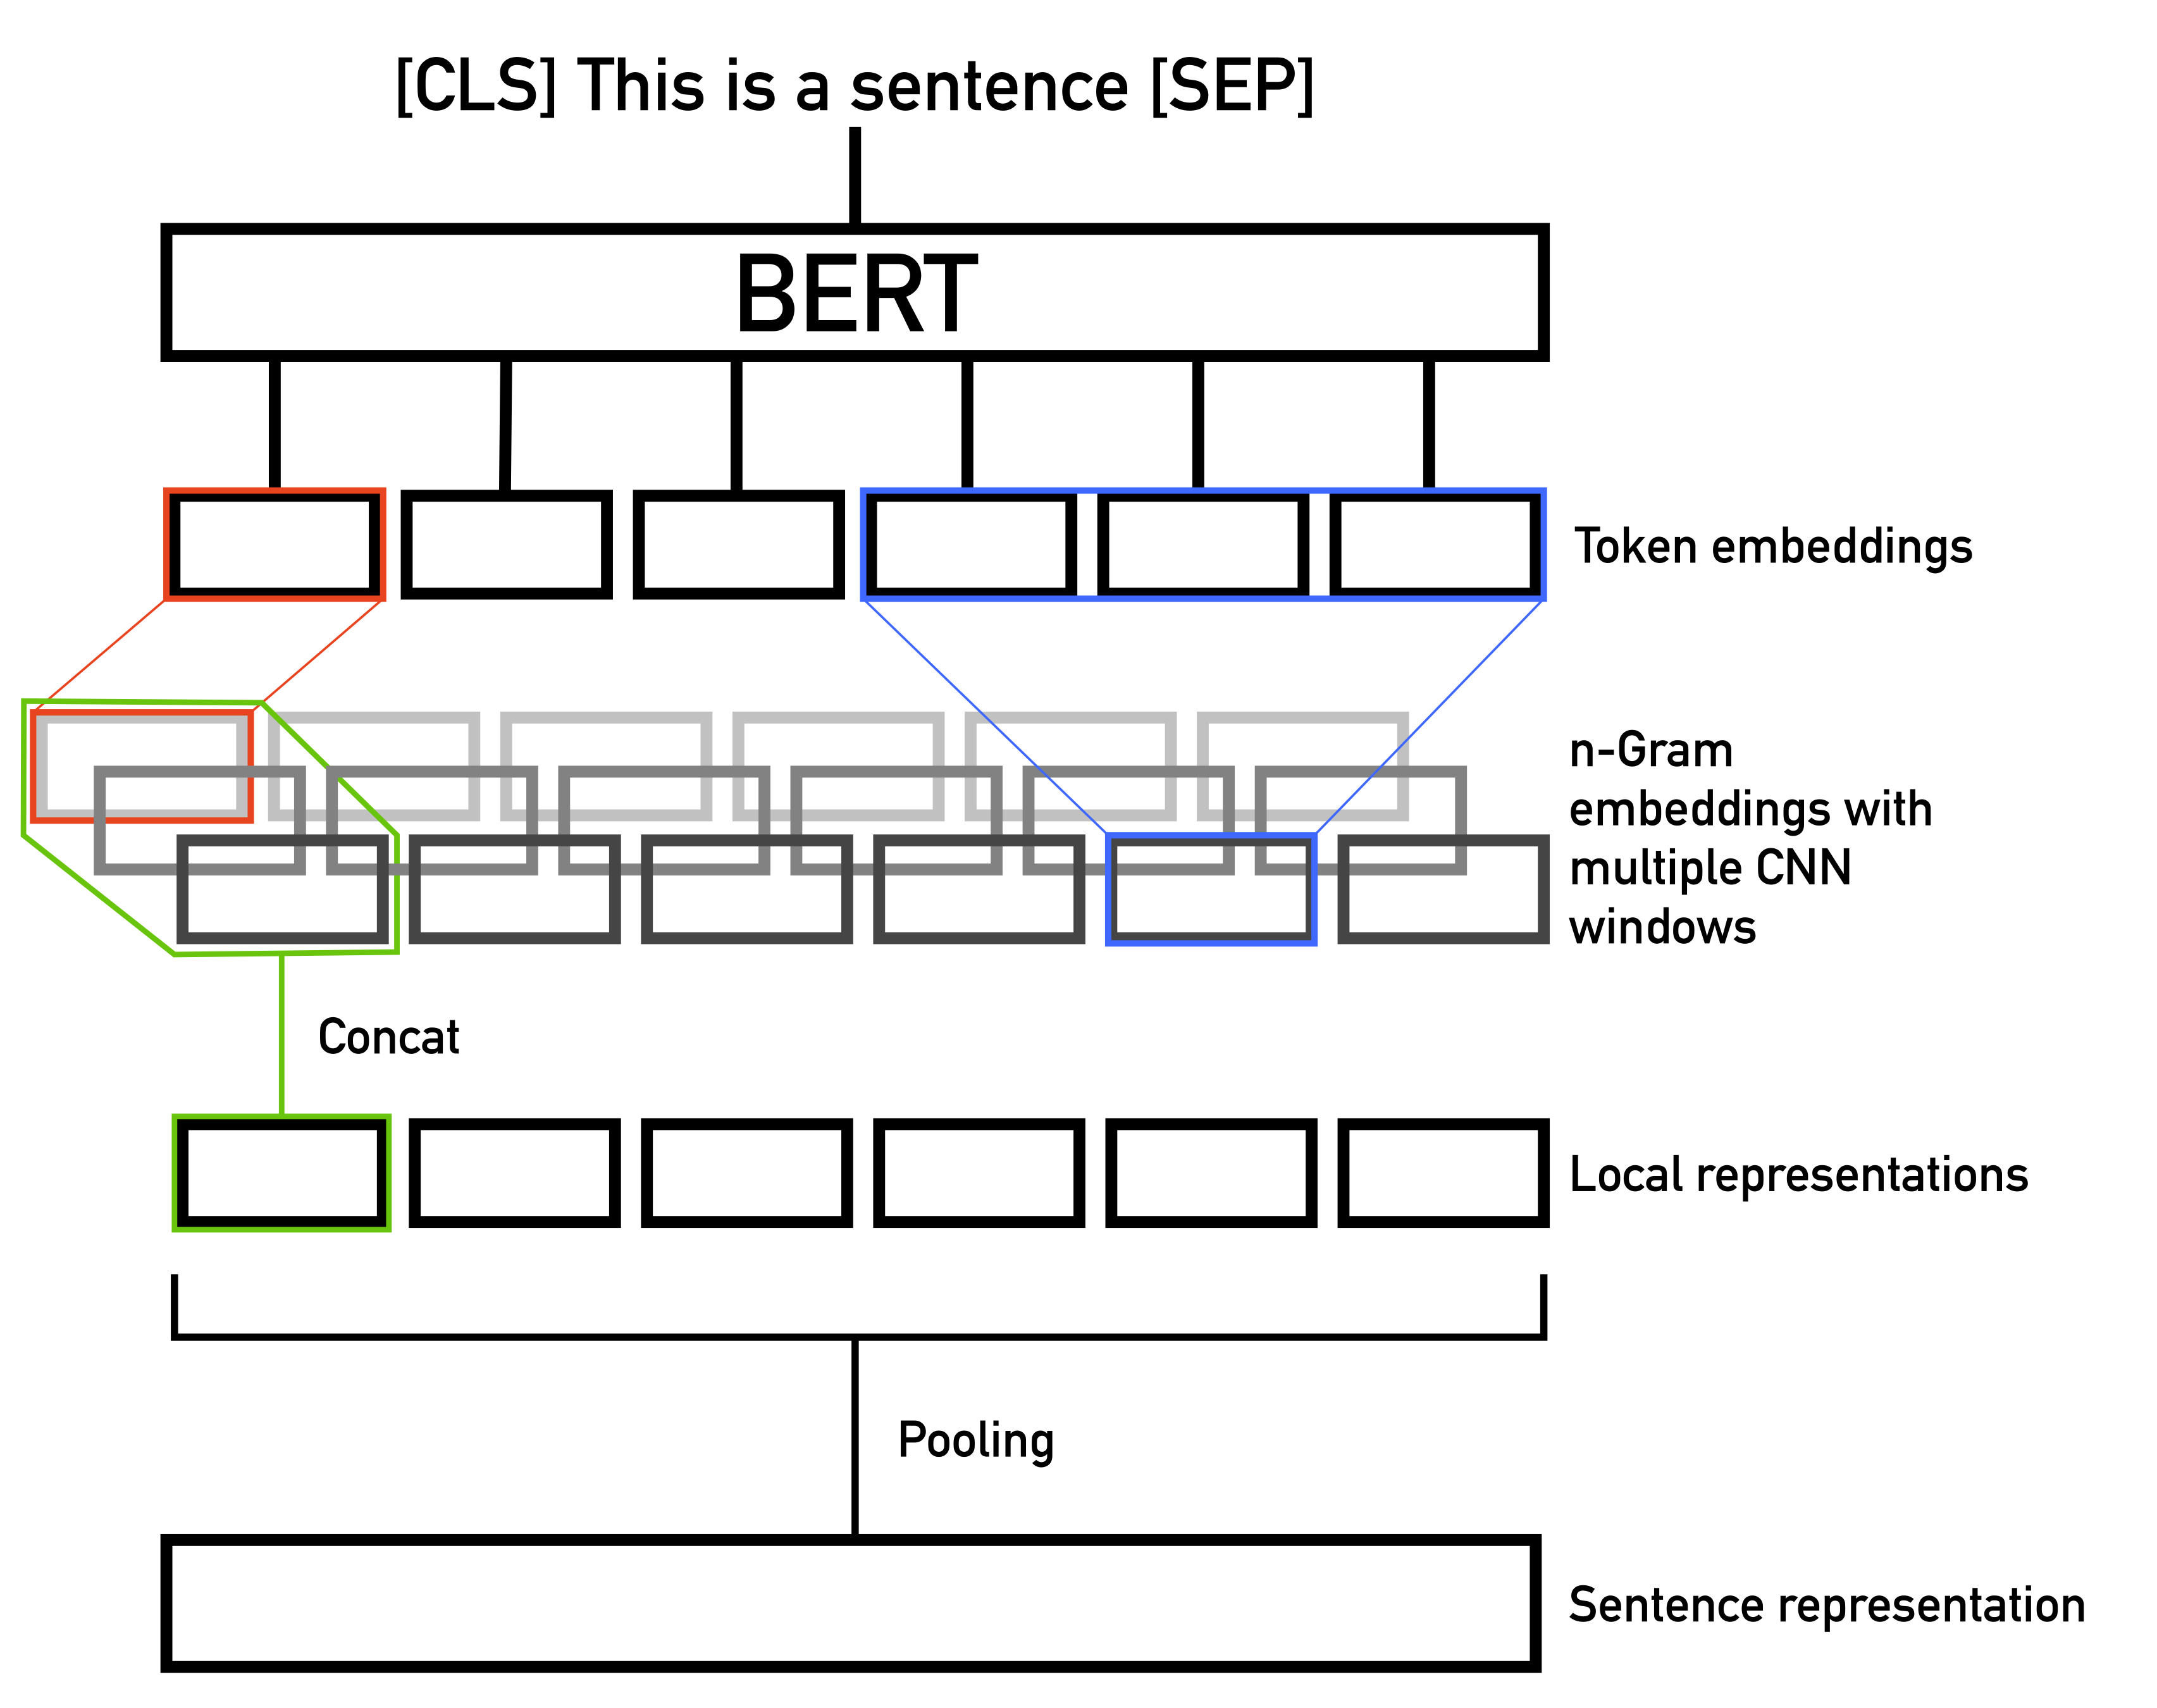
\includegraphics[width = 0.9\linewidth]{figures/IS-BERT1.png}
\caption{Process describing how to get the local context representations for IS-BERT}
\label{fig:local_context}
\end{figure}

But what are the local context representations? The process is illustrated in Figure \ref{fig:local_context}. The first step is to get the length-$l$ sequence of token embeddings $h_1, h_2, ..., h_l$ that can be obtained from BERT by encoding the input sentence. Multiple CNN layers with different kernel sizes are applied on top of these token embeddings. Different kernel sizes are used in order to be able to capture the different n-gram local contextual dependencies of the input sentence. The representations obtained with different window sizes are concatenated together to form one final local representation of a token ($\mathcal{F}^{(i)}_\theta(x)$, where $x$ is the input sentence and $i$ is the token index). To go from these token- to a sentence-representation, a mean-over-time pooling layer is used to create the global sentence representation $\mathcal{E}_\theta (x)$.

\begin{figure}[h!]
\centering
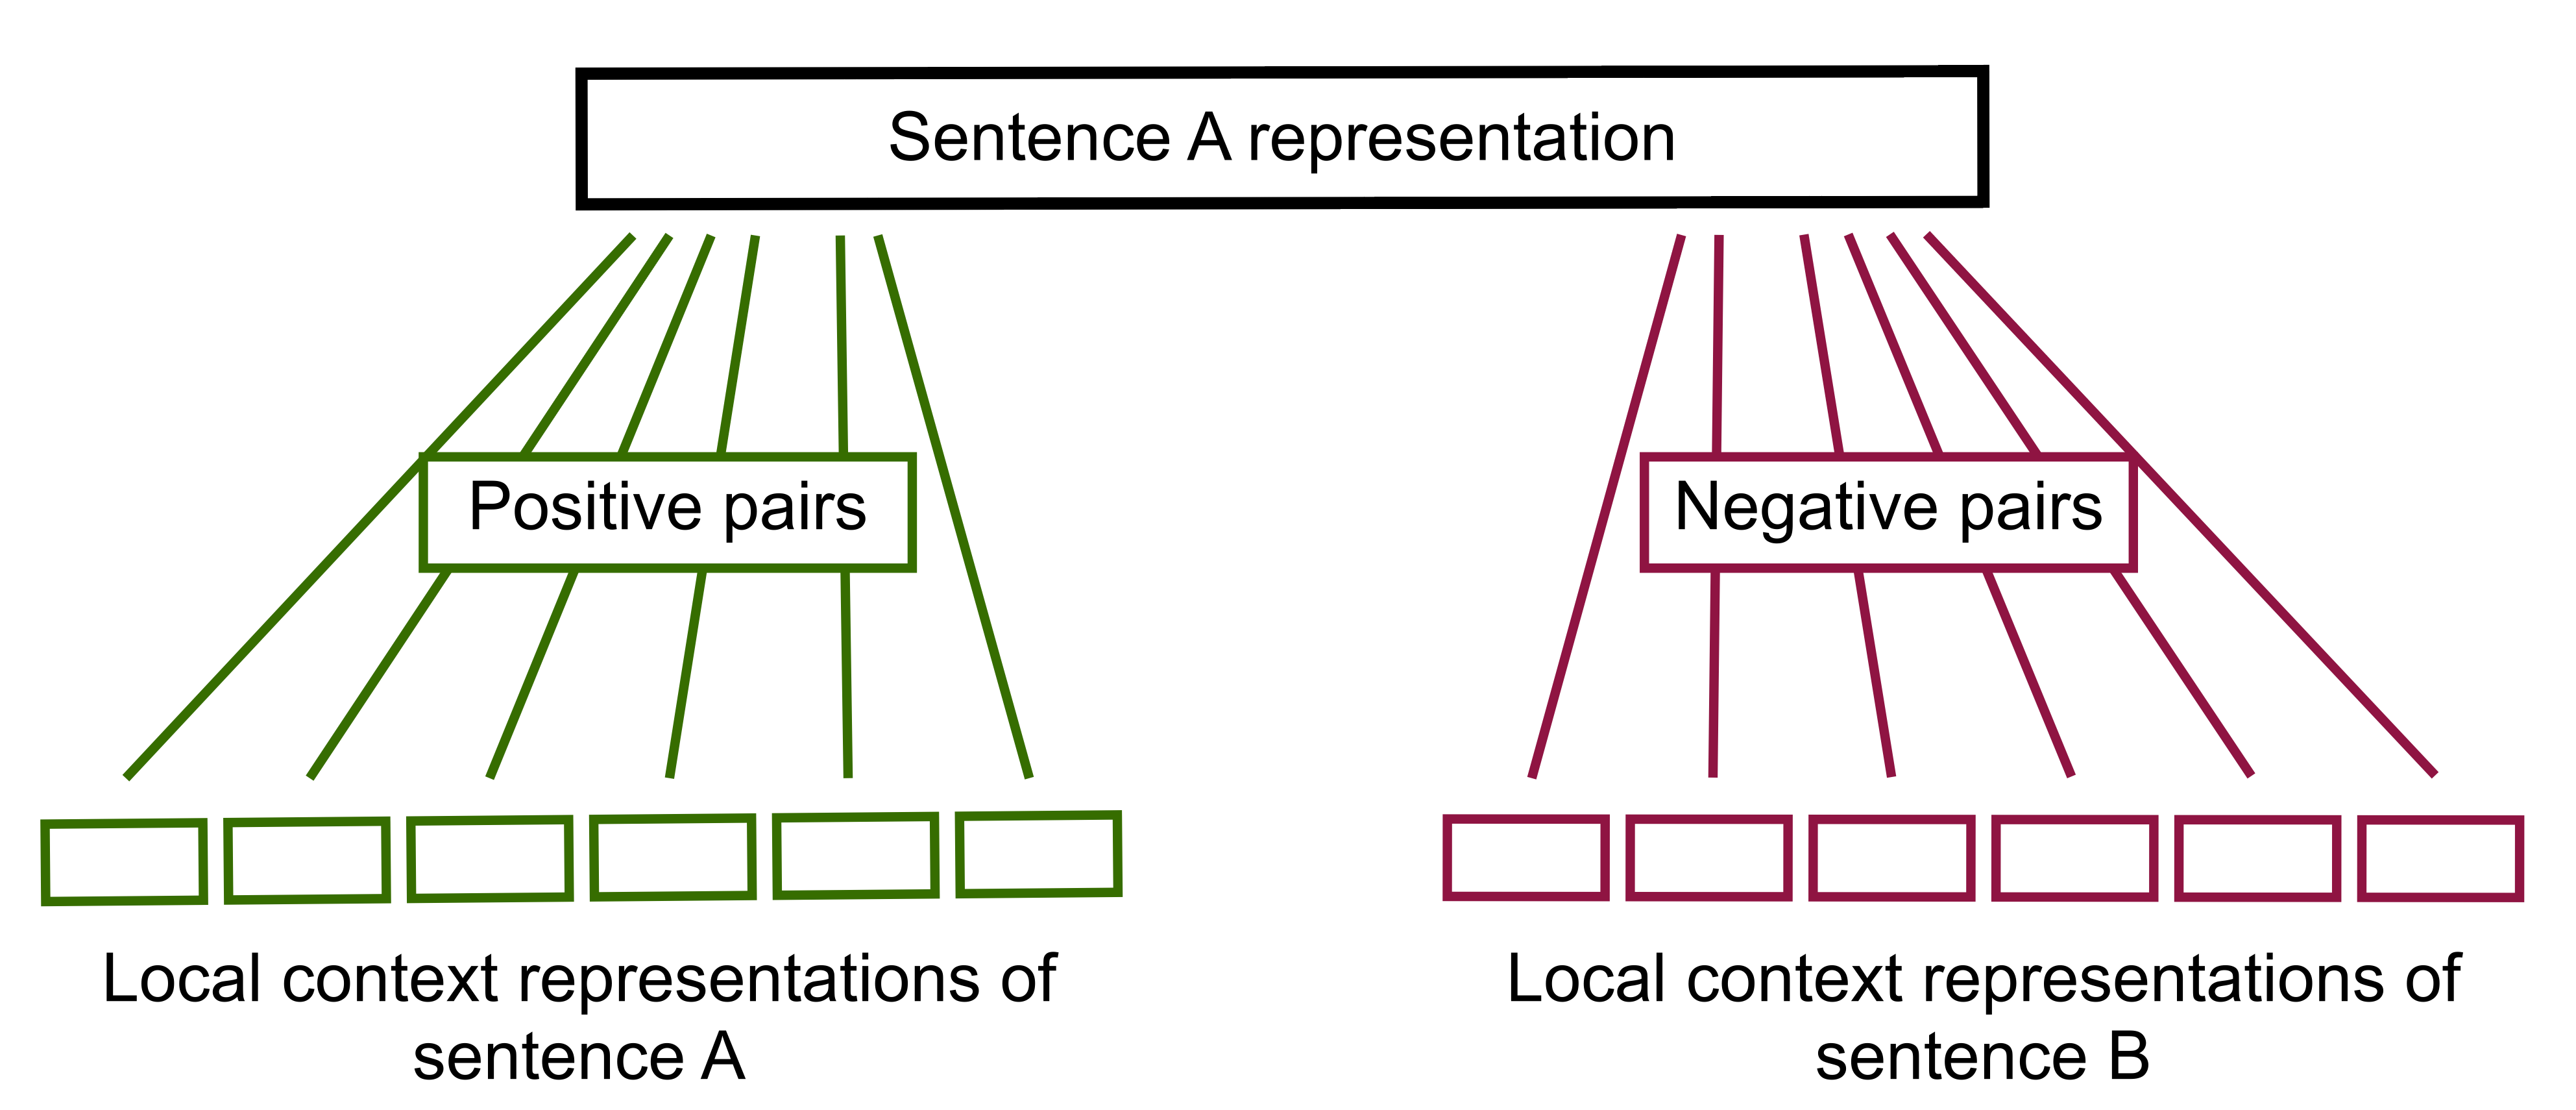
\includegraphics[width = 1\linewidth]{figures/IS-BERT2.png}
\caption{Contrastive learning in IS-BERT}
\label{fig:contrastive_learning}
\end{figure}

As mentioned before, the goal of contrastive learning is to maximize a similarity measure for positive pairs and minimize it for negative pairs. For IS-BERT, each sentence and its local context representations are treated as positive examples, and all the local context representations for other sentences are negative examples (as illustrated in Figure \ref{fig:contrastive_learning}). In \citet{zhang2020isbert} the similarity measure to estimate the mutual information between the global sentence representation $\mathcal{E}_\theta (x)$ and each of the local token representations $\mathcal{F}^{(i)}_\theta(x)$ is the Jensen-Shannon estimator. Maximizing it encourages the global sentence representation to have high mutual information with its own local context representations. As a consequence, the model will be driven to preserve the distinctive information that is shared by all local segments of the input sentence while remaining distinct from other sentences, resulting in expressive sentence representation \citep{zhang2020isbert}.

\section{Input Pattern Design}\label{input}

A model needs input in order to produce predictions. What this input is depends on the task. For NLP models, the inputs are words, sentences, or paragraphs. And in the case of the inputs in this thesis, it gets even more complex. The input has to contain different pieces of information (the party, the user query, and the context) that somehow have to be put together to be fed into the model. There is not one way to do this; instead, this is another part where experimentation is needed. Following is a brief overview of prompting and prefix design in general before Chapter \ref{experiments} goes over the different strategies utilized in this thesis.

\subsection{Prompting}

In recent years, there has been a great deal of interest and research in the area of prompting in NLP. Many of the current state-of-the-art LMs, such as GPT-3 \citep{brown2020gpt3} use prompting techniques to achieve their impressive performances. But what is prompting?

Prompting is the process of giving a stimulus or cue to a LM. A prompt is used to direct the model's generation process in a specific direction and can be in the form of a question, a statement, or a list of keywords. This can be done by reshaping the original task into a language modeling problem, a passage of text that has some unfilled slots. The LM then fills in the blanks, and that leads to the final output. For example: A model trained on general English data could be used to predict whether a review is positive or negative. To do this, the example sentence ``I did not have a good time.'' could be transformed into a prompt such as ``I did not have a good time. It was \underline{\hspace{1cm}}.'' The model then predicts something like ``terrible'', which indicates a negative review.

There are several benefits to using prompting in NLP. First and foremost, it can improve the performance of the model on a variety of tasks. By providing the model with a clear and relevant prompt, it is more likely to generate text that is accurate and useful. Prompting can also assist in lowering the amount of data needed to train a LM because, when given instructive prompts, the model can learn from fewer examples since it utilizes the general knowledge of language that a large pre-trained model has. A new task could be applied as few- or even zero-shot learning simply by using the right prompt. That makes fine-tuning much easier, faster, or even obsolete. Instead of trying to push the model to fit the data , the data is adjusted to suit the pre-trained model.

But that also means that the effectiveness of prompting relies on the model's ability to understand the context of the prompt and generate relevant and coherent responses. Without a good LM as its base, any prompt, however good, will not lead to good results. Picking the right prompts is one of the biggest challenges. A poorly constructed prompt may lead to false or irrelevant responses, which could harm the model's overall performance. Additionally, using prompts can introduce biases into the model because they might contain presumptions or preferences that have an impact on the results.

\subsection{Task Prefix} \label{task_prefix}

A versatile and effective method for fine-tuning big LMs is the use of task prefixes. That is what T5 \citep{raffel2020exploring} is doing, for example. Models can be trained to carry out a variety of NLP tasks by specifying a distinct prefix for each one, without significantly altering the model architecture or training procedure. The model determines the task it must carry out by examining the prefix at the beginning of the input sequence, and then it produces the appropriate output. By using the prefix ``sentiment analysis:'', for instance, a model could be trained to perform sentiment analysis on movie reviews. Input sequences that start with this prefix could then be categorized as either positive or negative, depending on the language used in the review. The same model could also be used to translate texts by utilizing the prefix ``translate English to German:'' followed by an English text.

The ability to simultaneously train a model on multiple tasks is one of the key benefits of using task prefixes. Using the same model for a variety of tasks like summarization, translation, and classification without them interfering with one another leads to increased efficiency and cost savings. Moreover, the ability to switch between tasks seamlessly without the need for retraining makes task prefixes an effective and adaptable NLP solution.


\subsection{Prompt Tuning}

So far prompts were text chosen by humans depending on what they think might work best. \citet{lester2021power} propose prompt tuning using so-called soft prompts. The LM is frozen, and instead the prompts are learned. The soft prompts are attached to the beginning of each embedded input and initialized at a fixed length. After each model iteration, the gradients calculated through back-propagation are only applied to these soft prompt vectors, keeping the core model the same. While that means that the prompts are not interpretable for humans, they still act in the same capacity as a manually written text prompt, but without being limited by discrete language.

The authors claim that their approach outperforms prompt design (tested on GPT-3 \citep{brown2020gpt3} and T5 \citep{raffel2020exploring}). Additionally, prompt tuning catches up to model tuning in terms of performance as model size grows. \citet{lester2021power} also show that soft prompting offers better transferability than full model fine-tuning in addition to parameter efficiency.

